\documentclass[prl,aps,reprint,noshowpacs,superscriptaddress,floatfix,letterpaper,longbibliography]{revtex4-2}
\usepackage{amsmath,amssymb,amsbsy,amsfonts,amsthm,bbm,bm,mathtools,mathrsfs}
\usepackage{color}
\usepackage{physics}
\usepackage{xfrac}
\usepackage[dvipsnames]{xcolor}
\definecolor{LapisLazuli}{RGB}{47, 102, 169}
\usepackage[colorlinks=true,citecolor=LapisLazuli,linkcolor=LapisLazuli,urlcolor=LapisLazuli]{hyperref}
\usepackage{empheq}
\usepackage{pgfplots}
\usepackage{stackengine}
\usepackage{relsize}
\usepackage[inline]{enumitem}
\usepackage[normalem]{ulem} % Comment this out before submitting papers! (otherrwsie will cause problems with references. 
\usepackage{comment}
\usepackage{import}
\usepackage[english]{babel}
\usepackage{lipsum}  

\renewcommand{\bibnumfmt}[1]{(#1)}
\usepackage{enumitem} 

% Macros
\newcommand{\sdc}[1]{\textcolor{blue}{[SD: #1]}}
\newcommand{\jrg}[1]{\textcolor{red}{#1}}
\newcommand{\jrgc}[1]{\textcolor{red}{[JRG: #1]}}
\newcommand{\PlaceHolder}{\blue{[TMP PLACE HOLDER]}} 

% Colors: 
\newcommand{\red}{\textcolor{red}}
\newcommand{\green}{\textcolor{green}}
\newcommand{\blue}{\textcolor{blue}}
\newcommand{\yellow}{\textcolor{yellow}} 
\newcommand{\magenta}{\textcolor{magenta}}

% Shortcuts
\newcommand{\speedtime}{\tau_{\!\scriptscriptstyle\mathcal{A}}} 
\newcommand{\speedtimework}{\tau_{\!\scriptscriptstyle\mathcal{W}}}
\newcommand{\Qdot}{\dot{\mathcal{Q}}}
\newcommand{\Wdot}{\dot{\mathcal{W}}}
\newcommand{\Q}{\mathcal{Q}}
\newcommand{\W}{\mathcal{W}}

% Bold letters
\newcommand{\bp}{\boldsymbol{p}}
\newcommand{\bq}{\boldsymbol{q}}
\newcommand{\bx}{\boldsymbol{x}}
\newcommand{\bC}{\boldsymbol{C}}

% Mathand Tables 
\newcommand{\cov}{\operatorname{cov}} % To mark covariance 
\newcommand{\Hquad}{\hspace{0.5em}} % Short spacing in equations
\newcommand{\HHquad}{\hspace{0.25em}} % Even shorter spacing 
\usepackage{pbox} % For breaking lines in table
\usepackage{tcolorbox}  % For a gray background textbox



\begin{document}
	
	\title{Paper title here}  
	
	\author{Author's name}
	\author{Jason~R.~Green}
	\email[]{jason.green@umb.edu}
	\affiliation{Department of Chemistry,\
		University of Massachusetts Boston,\
		Boston, MA 02125
	}
	\affiliation{Department of Physics,\
		University of Massachusetts Boston,\
		Boston, MA 02125
	}
	\date{\today}
	
\begin{abstract}	
	Abstract goes here.
	\lipsum[1-1]
\end{abstract}

\maketitle

\section{Introduction}
Introduction here Ref~\cite{Nicholson2020}

\lipsum[2-3]

\section{Results and Discussion}
Describe your results

\begin{align}
\Delta t \bar S/n&\geq k_B.\nonumber\\ 
&=\quad\text{Boltzmann's constant}\qquad >0\HHquad >1
\end{align}

\lipsum[2-3]
\begin{figure}[h!]
	\centering
	\hspace*{-0.75cm}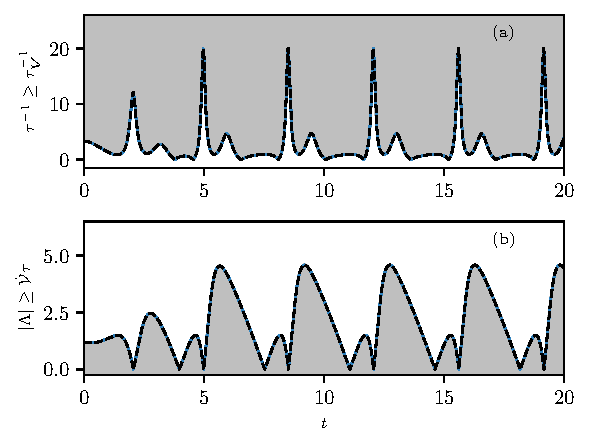
\includegraphics[width=0.45\textwidth]{sample-plot.pdf}
	\caption{Caption goes here}
	\label{fig:plot-label}
\end{figure}

\begin{figure}[t] 
\centering
\begin{tikzpicture}
\node (image) at (0,-0.125) {
  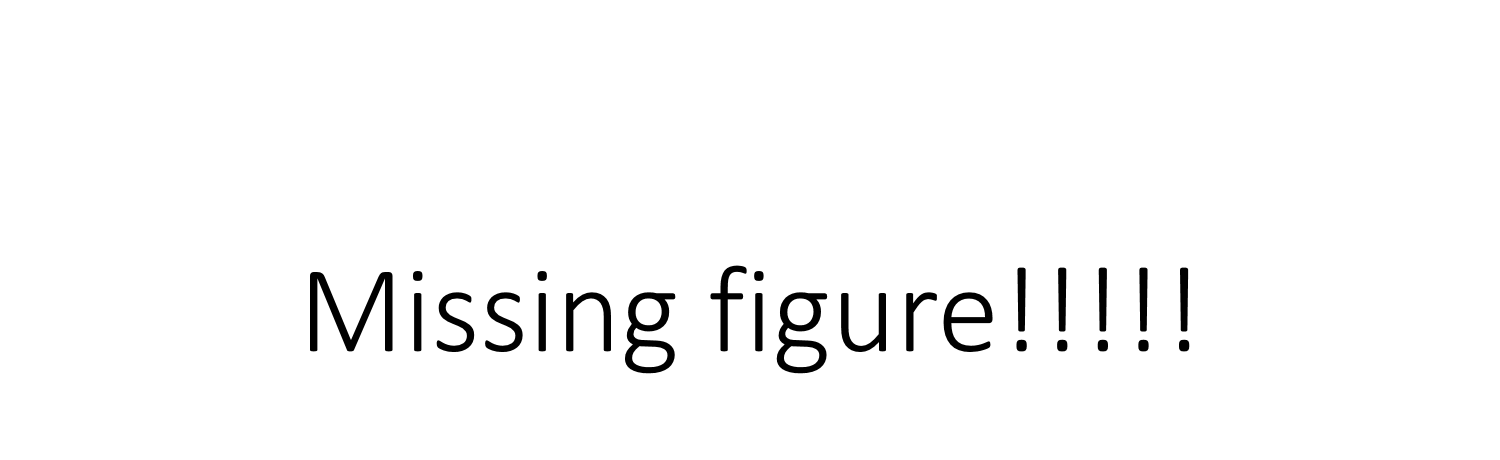
\includegraphics[width=0.9\linewidth]{Sample-tex-files/MissingFigure.png}
};
\node (image) at (0,-3.75) {
  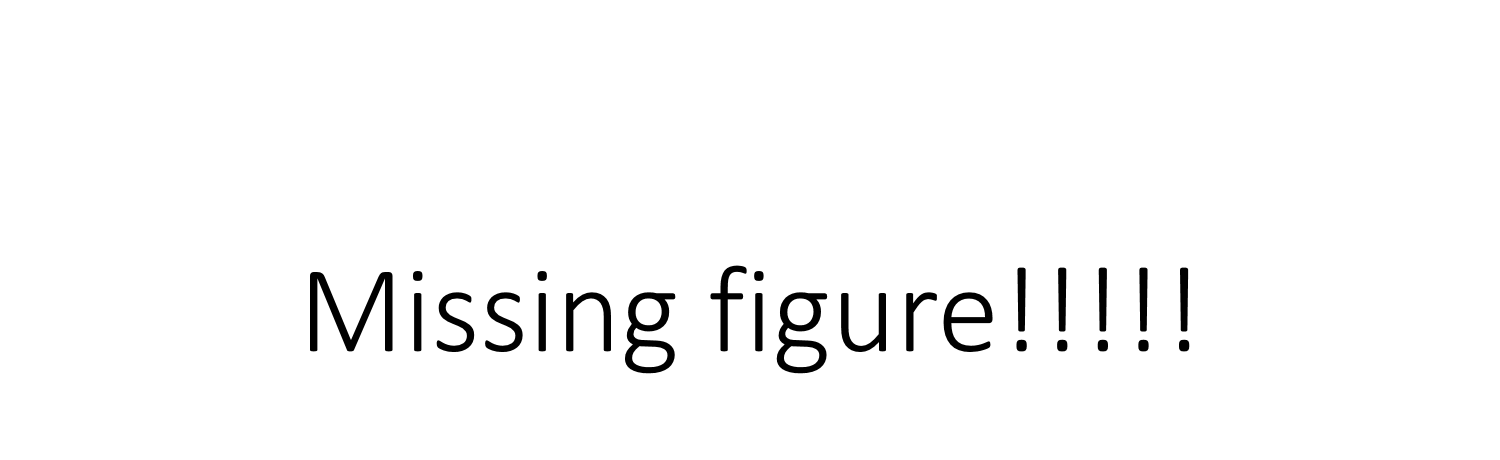
\includegraphics[width=0.9\linewidth]{Sample-tex-files/MissingFigure.png}
};
\node[text=black] (a) at (-2.3,1.4){\footnotesize{(a)}};
\node[text=black] (b) at (-2.3,-2.0){\footnotesize{(b)}};
\end{tikzpicture} 
\caption{
{\footnotesize{Figure with two panels, using Tikz.}}}
\label{fig:TikzExample} 
\end{figure} 


 %%%%%%%%% Start Table 
%\begin{widetext} 
%\begin{center}
\begin{table}[t] 
\footnotesize
%\centering 
\begin{tabular}{| c | c | c |} % (3 columns) 
\hline\hline 
Category & Col$1$ & Col$2$\\
[0.5ex] %
\hline 
Cat1&$1$&$2$\\
%%%%% 
Cat2&$1$&$2$\\
%%%%% 
Cat3&$1$&$2$\\
[0.5ex]
\hline\hline 
\end{tabular} 
\caption{\footnotesize{Example of a Table.}}
\label{Table1} 
\end{table} 
%\end{center} 
%\end{widetext}
%%%%%%%%% End Table 

\section{Conclusions}

Conclude the paper

\lipsum[2-3]
\\ 


\section{Acknowledgments}
\begin{acknowledgments}
% This text is provided by the funding agency. Jason will provide.
This material is based upon work supported by the National Science Foundation under Grant No. ....

\end{acknowledgments}

\appendix

\section{App. A}
\label{AppAT} 
We briefly explain the derivation of.... 
\begin{equation}
    (\text{This shows how Eqs in the App should be numbered.})
\end{equation}

\bibliography{references}

\end{document}
